\chapter{Triển khai ứng dụng}
\label{Chapter4}

\emph{Chương này sẽ trình bày, mô tả chi tiết về quá trình triển khai ứng dụng, kết quả phân tích bài toán chỉ đường, đưa ra các yêu cầu cụ thể cho bài toán. Đồng thời chương này cũng trình bày bản thế kế kiến trúc hệ thống và các thiết kế chi tiết khác.}

\section{Phân tích, đặc tả yêu cầu}

\subsection{Mô tả chung}
Sản phẩm là một ứng dụng cho phép người dùng ghi âm giọng nói hoặc nhập văn bản, sau đó tự phân tích giọng nói về văn bản để xác định yêu cầu và hướng dẫn đường đi. Sản phẩm cung cấp giao diện để người dùng có thể ghi âm và nhập văn bản trên ứng dụng di động một cách dễ dàng.
Mục đích của ứng dụng chatbot chỉ đường là cung cấp một giao diện thân thiện, người dùng có thể dễ dàng hỏi những câu hỏi liên quan đến đường đi bằng văn bản hoặc giọng nói và nhận câu trả lời ngay lập tức.
\subsection{Yêu cầu chức năng}

Yêu cầu chức năng chỉ đường từ một điểm đến một điểm bằng văn bản:
\begin{itemize}
    \item[--] Dữ liệu vào: Yêu cầu của người dùng dưới dạng văn bản
    \item[--] Xử lý: Thiết bị nhận văn bản để biết yêu cầu của người dùng. Nếu yêu cầu được hỗ trợ, hệ thống xử lý yêu cầu đó và phản hồi bằng giọng nói và văn bản cho người dùng. Nếu yêu cầu không được hỗ trợ, thiết bị phản hồi yêu cầu không được hỗ trợ bằng giọng nói và văn bản.
    \item[--] Kết quả: Phản hồi bằng văn bản hiển thị lên màn hình ứng dụng và giọng nói của thiết bị.
\end{itemize}
Yêu cầu chức năng chỉ đường từ một điểm đến một điểm bằng âm thanh (audio):
\begin{itemize}
    \item[--] Dữ liệu vào: Yêu cầu của người dùng dưới dạng audio
    \item[--] Xử lý: Thiết bị biến giọng nói vào thành văn bản để biết yêu cầu của người dùng. Nếu yêu cầu được hỗ trợ, hệ thống xử lý yêu cầu đó và phản hồi bằng giọng nói và văn bản cho người dùng. Nếu yêu cầu không được hỗ trợ, hệ thống phản hồi yêu cầu không được hỗ trợ bằng giọng nói và văn bản.
    \item[--] Kết quả: Phản hồi bằng văn bản hiển thị lên màn hình ứng dụng và giọng nói của thiết bị.
\end{itemize}

\subsection{Yêu cầu giao diện phần mềm}

Yêu cầu giao diện cho chức năng cho ứng dụng chỉ đường : Giao diện đơn giản, dễ sử dụng

Yêu cầu giao diện cho chức năng Chat chỉ đường bằng văn bản:
\begin{itemize}
    \item[--] Giao diện đơn giản, dễ sử dụng
    \item[--] Câu lệnh ngắn gọn, dễ ghi
    \item[--] Phản hồi ngắn gọn dễ nghe, dễ đọc
    \item[--] Phản hồi mọi câu lệnh dù câu lệnh đó không được hỗ trợ
\end{itemize}

Yêu cầu giao diện cho chức năng Chat chỉ đường bằng giọng nói:
\begin{itemize}
    \item[--] Giao diện đơn giản, dễ sử dụng
    \item[--] Câu lệnh ngắn gọn, dễ đọc
    \item[--] Phản hồi ngắn gọn, dễ nghe, dễ đọc
    \item[--] Phản hồi mọi câu lệnh dù câu lệnh đó không được hỗ trợ
    \item[--] Phải có giao diện ghi âm để phản hồi trực quan
\end{itemize}

\subsection{Yêu cầu hiệu suất}
\begin{itemize}
    \item[--] Thiết bị phải hoạt động được liên tục trong thời gian dài, từ 12 đến 24 giờ
    \item[--] Kết quả chỉ đường phải đạt độ chính xác tối thiểu 80\%
    \item[--] Tốc độ phản hồi phải nhỏ hơn 5 giây
    \item[--] Đảm bảo sự kết nối của nhiều ứng dụng cùng một thời điểm lên hệ thống
\end{itemize}

\subsection{Ràng buộc thiết kế}
\begin{itemize}
    \item[--] Sản phẩm phải được thiết kế bằng tiếng Việt, bao gồm giao diện người dùng, các phản hồi bằng giọng nói và văn bản
    \item[--] Sản phẩm ứng dụng cần đảm bảo tính thẩm mỹ
\end{itemize}

\subsection{Ràng buộc thuộc tính}
\begin{itemize}
    \item[--] Cần đảm bảo việc kết nối và tương tác nhiều ứng dụng lên hệ thống
    \item[--] Việc cập nhật phần mềm phải nhanh chóng và không gây ra mất mát dữ liệu
\end{itemize}

\section{Thiết kế kiến trúc hệ thống}
Phần mềm hệ thống gồm ba nhóm (xem hình Kiến trúc hệ thống \ref{fig:kien-truc-he-thong}):
\begin{itemize}
    \item[--] Phần mềm chạy trên thiết bị di động
    \item[--] Máy chủ
    \item[--] \ac{api}
\end{itemize}
\begin{figure}[htp]
    \centering
    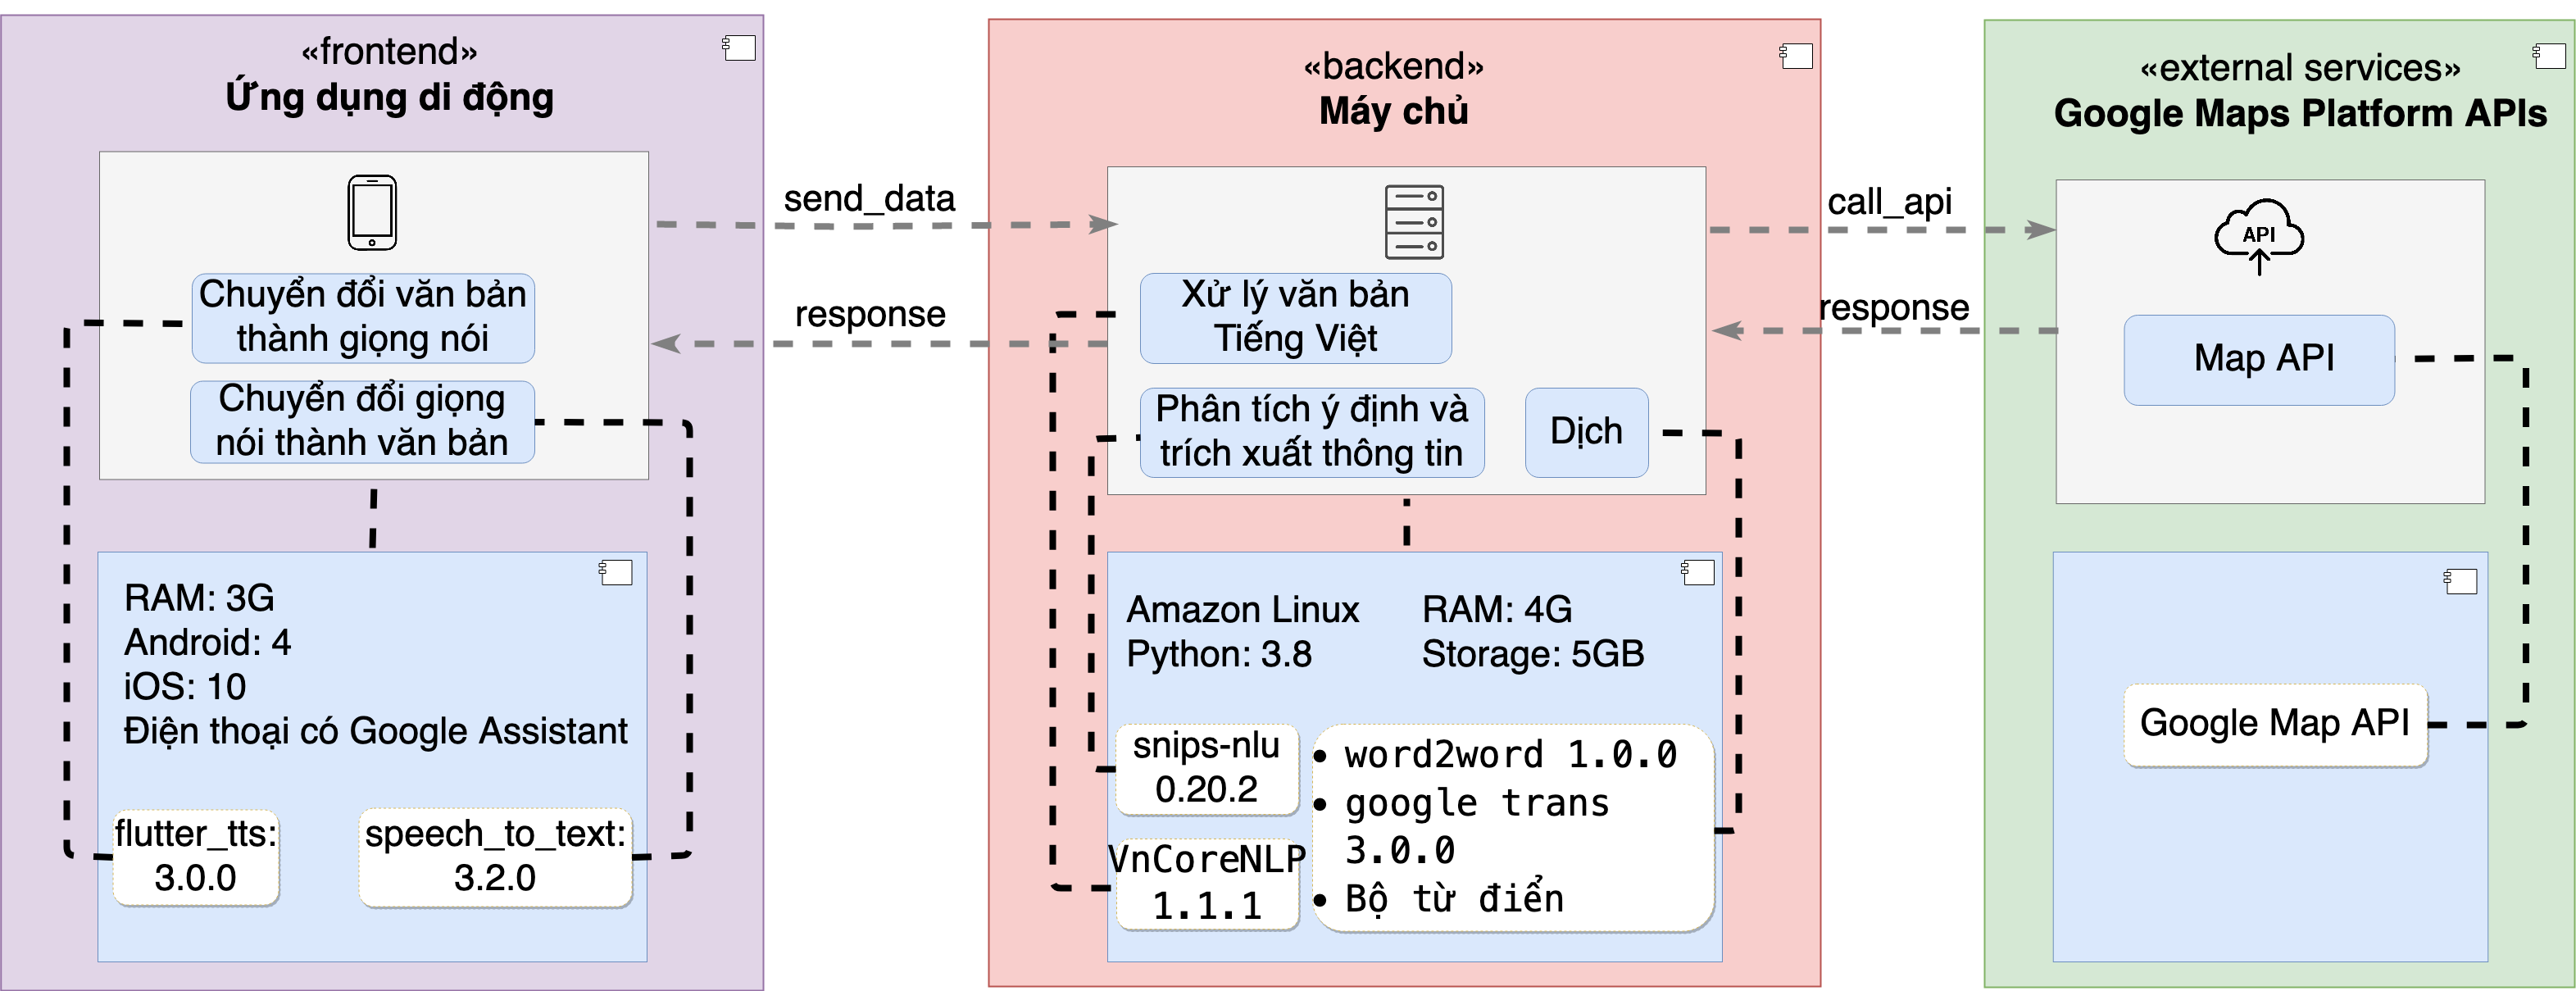
\includegraphics[width=10cm]{images/Structure-System.png}
    \caption{Kiến trúc hệ thống}
    \label{fig:kien-truc-he-thong}
\end{figure}

Máy chủ (Server) thực hiện chương trình xử lý và phân tích dữ liệu. Chương trình này chịu trách nhiệm xử lý dữ liệu gửi lên (Text) bao gồm thành phần: Phân tích ý định, trích xuất dữ liệu và tìm kiếm kết quả trả lời câu hỏi của người gửi. Khi ứng dụng điện thoại gửi Text lên, chương trình xử lý rồi trả về kết quả trên ứng dụng điện thoại. Máy chủ sẽ cung cấp các API tương ứng. Các API cung cấp giao diện cho phép app di động giao tiếp với chương trình xử lý ở máy chủ.

Trong phạm vi đề tài, nhóm sẽ xây dựng thành phần xác định ý định, trích xuất dữ liệu và tìm kiếm kết quả trả lời câu hỏi sẽ sử dụng API của Google Map\cite{google-map}. 

Phầm mềm ứng dụng cung cấp một giao diện người dùng qua ứng dụng trên điện thoại di động. Giao diện này cho phép người dùng sử dụng để hỏi các câu hỏi về chỉ đường từ một địa chỉ này đến một địa chỉ khác cụ thể bằng giọng nói (ghi âm câu nói) hoặc là nhập văn bản trên ứng dụng và trả về cho người dùng kết quả phù hợp.
\begin{itemize}
    \item[--] Chuyển giọng nói thành văn bản: Chuyển câu lệnh bằng giọng nói của người dùng thành văn bản để hiển thị lên ứng dụng và gửi lên hệ thống.
    \item[--] Chuyển văn bản thành giọng nói: Chuyển phản hồi của hệ thống thành dạng âm thanh để phát ra qua điện thoại.
\end{itemize}

Hai thành phần chuyển giọng nói thành văn bản và chuyển văn bản thành giọng nói được thực hiện ở ứng dụng di động bằng cách sử dụng package SpeechToText \footnote{Xem thêm về SpeechToText \url{https://pub.dev/packages/speech_to_text}} và TextToSpeech\footnote{Xem thêm về TextToSpeech \url{https://pub.dev/packages/flutter_tts}} do Flutter cung cấp.

\section{Xây dựng thành phần xác định ý định và trích xuất thực thể}
\subsection{Tạo dữ liệu tiếng Việt}
Nhóm đã thực hiện tạo dữ liệu gồm hai intent là findRoute và askLocation. Mỗi intent gồm 20 câu huấn luyện và 10 câu để kiểm thử.
\begin{itemize}
    \item[--] Tạo dữ liệu trên file txt. Với intent "findRouteAB" ta có câu ví dụ: "Đường đi từ đại học Sài gòn đến Cao đẳng sài gòn"
    \item[--] Chuyển dữ liệu sang dạng json để thuận tiện cho việc huấn luyện (Xem hình dữ liệu dưới dạng file json \ref{fig:data-train-json} ).
\end{itemize}
\begin{figure}[htp]
    \centering
    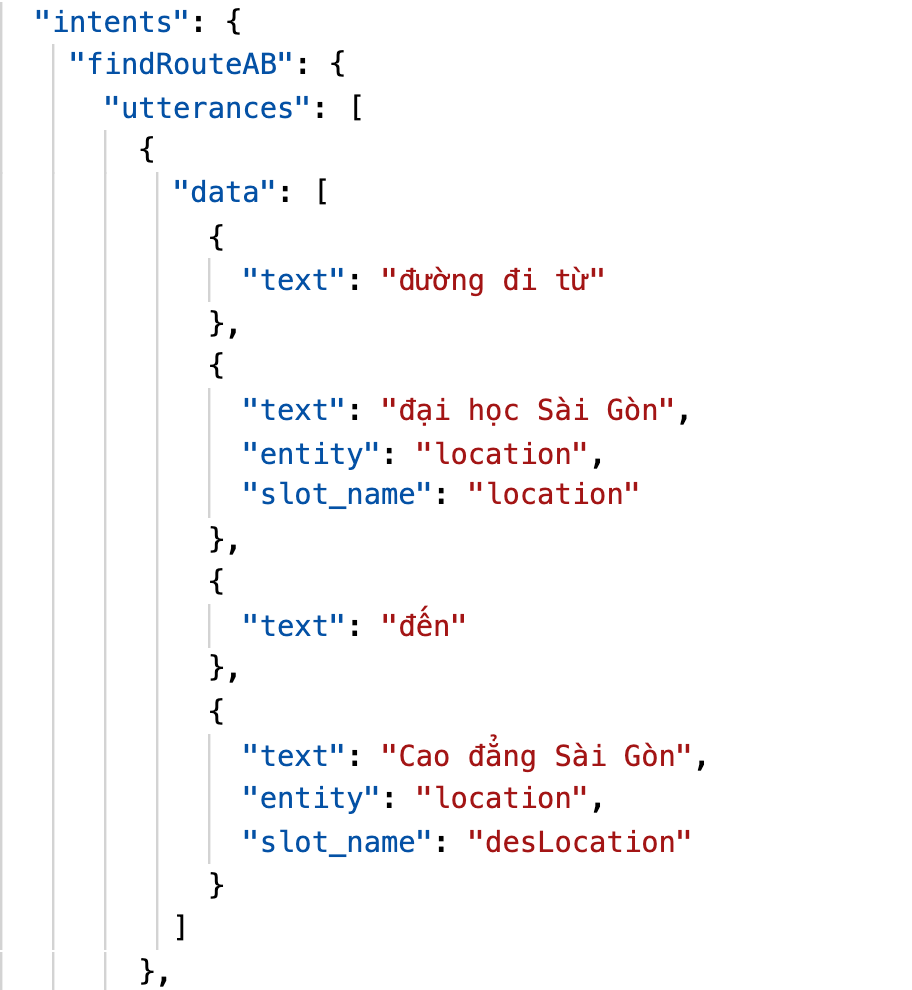
\includegraphics[width=10cm]{images/Data-train-json.png}
    \caption{Hình ảnh minh họa dữ liệu trước khi dịch và sau khi dịch}
    \label{fig:data-train-json}
\end{figure}

\subsection{Huấn luyện dữ liệu và kết quả}

Thông qua kết quả của quá trình thực hiện chuyển hoá dữ liệu từ tiếng Việt sang tiếng Anh để chuẩn bị dữ liệu cho quá trình huấn luyện mà chúng em đã tiến hành nghiên cứu, chúng em nhận thấy kết quả của việc "Xây dựng bộ từ điển" cho riêng ứng dụng theo các chủ đề, lĩnh vực cụ thể đem lại hiệu quả tốt trong quá trình dịch và không làm sai lệnh ngữ nghĩa của câu. Vì vậy chúng em chọn giải pháp "Xây dựng bộ từ điển" để thực hiện chuyển hoá dữ liệu sang tiếng Anh để tiến hành thực hiện huấn luyện dữ liệu.

Chúng em đã tiến hành dịch toàn bộ dữ liệu huấn luyện sang tiếng Anh với ... câu và ... câu test. Trong đó, dữ liệu huấn luyện chi tiết cho mỗi intent như sau: 

\begin{itemize}
    \item[--] Đường đi từ một địa điểm đến một địa điểm - "findRouteAB": Huấn luyện với ... câu và ... câu test.
    \item[--] Hỏi vị trí hiện tại - "askLocation": Huấn luyện với ... câu và ... câu test.
\end{itemize}

Đem bộ dữ liệu để huấn luyện và đánh giá, ta đạt được kết quả như hình \ref{fig:sodohethongchiduong}, xem chi tiết \footnote{\url{https://drive.google.com/file/d/1HSe-ri76d8jbF3FZUCrDiFawHI17D18a/view?usp=sharing}}:

\begin{figure}[htp]
    \centering
    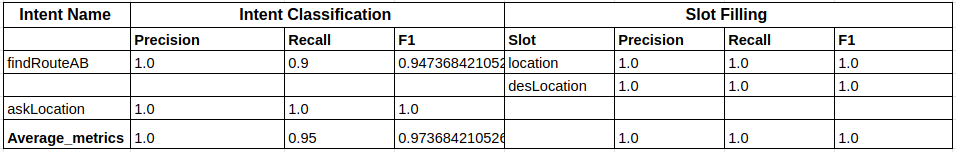
\includegraphics[width=15cm]{images/metrics-tudien.png}
    \caption{Các chỉ số của mô hình}
    \label{fig:sodohethongchiduong}
\end{figure}
